\chapter{Lösen von ODEs mittels stückweiser Linearisierung}

\section{Verallgemeinerte Mittelpunktsregel}

Unser Ziel ist es nun, ausgehend von der wohlbekannten Impliziten Mittelpunktsregel
\[
 \xhat  = \xcheck + hF\left( \frac{\xhat + \xcheck}{2}\right)
\]
die im vorherigen Kapitel hergeleitete stückweise Linearisierung zur Lösung von ODEs mit verketteter stückweise glatter rechter Seiten anzuwenden.
Hierbei ist $\xhat = x(h)$ und $\xcheck = x(0)$.

Gegeben sei eine gewöhnliche Differentialgleichung
\[
 \dot x = F(x(t))
\]
mit verkettetem stückweise glattem und global Lipschitzstetigem $F$. Mit dem Hauptsatz der Differential- und Integralrechnung folgt
\[
 \xhat - \xcheck = \int_0^h F(x(t)) \text{d}t
\]
und mit $t = \frac{h}{2} + \tau h$ als Substitution ergibt sich
\[
 \xhat - \xcheck = h\int_{-\sfrac{1}{2}}^{\sfrac{1}{2}} F\left(x \left(\sfrac{h}{2} + \tau h\right)\right) \text{d}\tau
\]
Da das Integral in den Grenzen $-\sfrac{1}{2}$ und $\sfrac{1}{2}$ liegt, stellt $\sfrac{h}{2}$ den Mittelpunkt des Integrationsgebietes dar. Durch Approximation von $x(t)$ durch die Sekante $(\frac{1}{2} - \tau) \xcheck + (\frac{1}{2} + \tau) \xhat$ folgt:
\[
 \begin{aligned}
 \xhat - \xcheck & = h\int_{-\sfrac{1}{2}}^{\sfrac{1}{2}} F\left(\frac{\xcheck + \xhat}{2} + \tau (\xhat - \xcheck)\right) \text{d}\tau + \mathcal O(h^3)
 \end{aligned}
\]
Nun schätzen wir die rechte Seite $F(\ldots)$ durch seine stückweise Linearisierung ab und erhalten schließlich
\[
 \xhat -  \xcheck = h\int_{-\sfrac{1}{2}}^{\sfrac{1}{2}} F(\xo) + \Delta F(\xo;\tau (\xhat - \xcheck))  \text{d}\tau + \mathcal O(h^3)
\]
die von Griewank in \cite[S.21 (14)]{monster} eingeführte verallgemeinerte Implizite Mittelpunktsregel
\begin{equation}
 \xhat -  \xcheck = h\int_{-\sfrac{1}{2}}^{\sfrac{1}{2}} F(\xo) + \Delta F(\xo;\tau (\xhat - \xcheck))  \text{d}\tau
\end{equation}

Da sowohl die Approximation durch Sekanten als auch der stückweisen Linearisierung einen Fehler von $\mathcal O(h^2)$ bzgl. der exakten Lösung $x(t)$ besitzen und das Integral $h$ als Multiplikator besitzt ergibt sich letztendlich ein Fehler dritter Ordnung.

Der Vorteil der Formel besteht darin, dass sie konsistent zur Impliziten Mittelpunktsregel ist. Falls $F$ nämlich glatt ist, so kommt die Auswertungsprozedur für $\Delta F(\xo;\tau (\xhat - \xcheck))$ ohne die Regel \eqref{eq:absAdRule} aus und es gilt 
\[
 \Delta F(\xo;\tau (\xhat - \xcheck)) = F'(\xo) \tau (\xhat - \xcheck)
\]
Das bedeutet, dass
\begin{equation}
\begin{aligned}
   \xhat -  \xcheck &= h\int_{-\sfrac{1}{2}}^{\sfrac{1}{2}} F(\xo) + \Delta F(\xo;\tau (\xhat - \xcheck))  \text{d}\tau\\
		    &= h\int_{-\sfrac{1}{2}}^{\sfrac{1}{2}} F(\xo) + F'(\xo)\tau (\xhat - \xcheck))  \text{d}\tau\\
		    &= h F(\xo)
\end{aligned}
\label{eq:equivalenceGenImplMidpoint}
\end{equation}

Damit ist die verallgemeinerte Implizite Mittelpunktsregel eine echte Verallgemeinerung der bekannten Impliziten Mittelpunktsregel. 
Griewank bewies in \cite[Prop.4]{monster} ihre Konvergenzeigenschaft
\begin{theorem}[Konvergenz verallg. Impl. Mittelpunktsregel]
 Angenommen, $F$ sei eine verkettete stückweise glatte Funktion und Lipschitzstetig in einer offenen Umgebung $\mathcal D$ des Ursprungs $\xcheck =0$. Dann existiert eine obere Schranke $\bar h>0$, sodass für alle $h<\bar h$ die Funktion 
 \[
    hG(x) = h\int_{-\sfrac{1}{2}}^{\sfrac{1}{2}} F(\xo) + \Delta F(\xo;\tau (\xhat - \xcheck))  \text{d}\tau
 \] 
 eine abgeschlossene Kugel $B_\rho(0)\subset \mathcal D$, $\rho>0$ in sich selbst abbildet und kontraktiv ist.
 Desweiteren genügt der eindeutige Fixpunkt $x_h\in B_\rho(0)$
 \[
  x_h - x(h) = \mathcal O(h^3)
 \]
  wobei $x(t)$ die Gleichung $\dot x(t) = F(x(t))$ mit  $x(0)= 0$ löst.
\end{theorem}

Für den von Boeck \cite{boeck14} hergeleiteten Algorithmus benötigen wir zum einen die Möglichkeit eine stückweise lineare Funktion möglichst genau in einem Intervall zu integrieren als auch ein Löser für Lineare Gleichungssysteme.
% Dies wird im nächsten Abschnitt behandelt.

\section{Quadratur und Unfoldeded Newton}
\subsection{Quadraturverfahren}

Die Aufgabe besteht nun darin, eine stückweise lineare Funktion $F:\R^n \to \R^m$ genau zu integrieren. Dazu sei die stückweise Linearisierung $F(\xo) + \Delta F(\xo,\Delta x)$ mit einer Richtung $\Delta x$ als Abs-Normal Form gegeben, wie sie in Abschnitt \ref{sec:absNormalForm} eingeführt wurde. 
Für unser Problem ist es ausreichend, nur $\Delta F(\xo,\Delta x)$ zu betrachten, da $F(\xo)$ konstant ist.
Nehmen wir an, das in dem Integrationsgebietes des Integrals
\begin{equation}
\label{eq:quadInitialProblem}
 \int_0^{\sfrac{1}{2}} \Delta F(\xo,t\Delta x) \text{d}t
\end{equation}
$k$ Kinks des Integranten vorhanden sind. 
%Kink Berechnung
Um diese Kinks aus der Abs-Normal Form zu berechnen, werden die switching Variablen $z_j$, $j=1,\dots,s$ aus der Abs-Normal Form betrachtet. Wie bereits in Kapitel \ref{sec:absNormalForm} erwähnt sind diese Werte für sich genommen stückweise affine Funktionen, an deren Nullstellen ein Kink auftritt,
d.h. an ihren Nullstellen findet ein Vorzeichenwechsel statt. Um zu wissen, wie weit wir von einem Punkt $\xo$ in Richtung $\Delta x$ gehen können bis wir solch eine Nullstelle erreichen, wollen wir diese \textit{kritischen Multiplikatoren} $\tau_j$, $j=1,\ldots, s$ berechnen. 
%Quadraturbeschreibung blub
\begin{figure}[H]
\centering
 \documentclass{standalone}
\usepackage{pgfplots,pgfplotstable}

\usetikzlibrary{external}

\begin{document}

\tikzsetnextfilename{multiple_kinks}
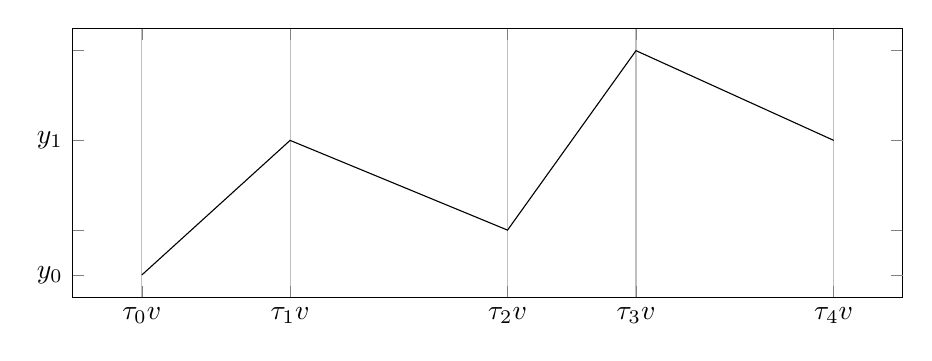
\begin{tikzpicture}
% \draw (0,0) grid (7,3);
% \draw[help lines,->] (0,0) -- (7,0) node[anchor=north west] {$v$};
% \draw[help lines,->] (0,0) -- (0,3) node[anchor=south east] {$y$};
% 
% \draw (0,1) -- (1,2) -- (2,0.5) -- (3,1.5) -- (4,1) -- (5,2.5) -- (6,2);
\begin{axis}[
	width=\textwidth,
	height=5cm,
% 	xlabel = $v$,
% 	ylabel = $y$,
	xtick = data,
	ytick = data,
	xmajorgrids,
	xticklabel={$\tau_{\pgfmathprintnumber{\ticknum}}v$},
	yticklabel=\empty,
	extra y ticks={1,1.3},
	extra y tick labels={$y_0$,$y_1$},
]
	\addplot[no marks] table {
		0 1
		1.5 1.3
		3.7 1.1
		5 1.5
		7 1.3
	};
\end{axis}

\end{tikzpicture}

 
\end{document}

 \caption{Quadratur zwischen mehreren Kinks}
\label{fig:quadrature} 
\end{figure}
\subsubsection{Kritische Multiplikatoren}
Dafür nehmen wir die erste Zeile der Abs-Normal-Form \eqref{eq:absNormalForm}
\begin{equation}
\label{eq:absNormalZ}
 z = c+Zx + L|z|
\end{equation}
und deren Richtungsableitung an $z$
\begin{equation}
\label{eq:absNormalZDerivative}
 \dot z = Z\Delta x + L\Sigma \dot z, \quad
 \Sigma  = \diag(\sigma(z)) ~ \text{mit } \sigma_j =  \begin{cases}
            \sign(z_j) & \text{falls } z_j\neq 0\\
            \sign(\dot z_j) &  \text{sonst}
           \end{cases}
\end{equation}

und bilden für jedes $z_j$ seine Tangente
\[
 z_j + \tau \dot z_k = 0 \quad \Leftrightarrow \quad \tau =- \frac{z_k}{\dot z_k}
\]
deren Nullstelle wir berechnen. Da sich das Vorzeichen des Abs Aufrufs in \eqref{eq:absNormalZ} bis zur Nullstelle nicht ändert, wir uns also im selben Polyeder befinden, haben wir lokal eine affine Funktion, deren Richtungsableitung \eqref{eq:absNormalZDerivative} lokal wohldefiniert ist.
Falls $z_j\dot z_j <0$ gilt, kreuzt die Tangente in Richtung $\Delta x$ einen Kink.
Der kritische Multiplikator $\tau_*$ ergibt sich dann als das Minimum der errechneten Werte oder im Falle, dass kein Kink vorhanden ist als obere Integrationsgrenze
\[
 \tau_* = \min \begin{cases}
		\frac{1}{2}\\
		\inf_j\lbrace -\frac{z_j}{\dot z_j}~ \vert ~ \dot z_j \cdot z_j <0 \rbrace
	       \end{cases}
\]

%Quadraturbeschreibung blub
\begin{figure}
\centering
 \documentclass{standalone}
\usepackage{pgfplots,pgfplotstable}

\usetikzlibrary{external}

\begin{document}

\tikzsetnextfilename{finding_kinks}
\begin{tikzpicture}[x=1.7cm,y=1.7cm]
\draw[->] (0,-.2) -- (0,2.5);
\draw[->] (-.2,0) -- (2.5,0);
\draw[] (-.2,2.2) -- (2.2,-.2) 
node[sloped,pos=0.5,anchor=north] {$z_j + \tau_j \dot z_j$};
% \draw[decorate,decoration={brace,raise=4pt}] (0,2) -- (2,0) 
% node[pos=0.5,anchor=south west] {$\tau$};
\draw[] (-.1,2) -- (.1,2);
\draw (2,-.1) -- (2,.1);
\node[] at (-.3,2) {$z_j$};
\node[pos=0,anchor=north east] {$0$};
\end{tikzpicture}

 
\end{document}

 \caption{Kink- Berechnung}
\label{fig:findingKinks} 
\end{figure}

Nun, da wir die Stellen der $k$ Kinks ausrechnen könnne, teilen wir das Intervall $[0,\frac{1}{2}]$ in $k$-Abschnitte mit reellen Zahlen $0=\tau_0<\tau_1<\ldots<\tau_k = \sfrac{1}{2}$,  sodass
\[
 [0,\sfrac{1}{2}] = \bigcup_{i=0}^{k-1} [\tau_i,\tau_{i+1}]
\]
damit wir das Integral zerlegen können in
\[
 \int_0^{\sfrac{1}{2}} \Delta F(\xo,t\Delta x) \text{d}t = \sum_{i=0}^{k-1} \int_\tau^{\sfrac{1}{2}} \Delta F(\xo,t\Delta x) \text{d}t
\]
Mit $y_i = \Delta F(\xo;\tau_i \Delta x)$ und $F$ stückweise linear folgt, dass sich die Quadratur \ref{eq:quadInitialProblem} zu
\begin{equation}
\begin{aligned}
 \int_{\tau_{i-1}}^{\tau_i} \Delta F(\xo;t\Delta x) \text{d}t &= \int_{\tau_{i-1}}^{\tau_i}\left[ y_i+ \frac{y_{i+1}-y_i}{\tau_{i+1}-\tau_i}(t-\tau_i) \right] \text{d}t \\
 &=\frac{1}{2}(\tau_{i+1} -\tau_i)(y_{i+1}-y_i)
 \end{aligned}
\end{equation}
vereinfacht, also zur Trapezregel. Für stückweise lineare Funktionen ist die eben beschriebene Integrationsmethode exakt, da die Trapezregel für lineare Funktionen exakt ist.
Mit dem Algorithmus in Prozedur \ref{alg:quad} kann nun die Quadratur für stückweise lineare Funktionen berechnet werden. 
\begin{algorithm}[H]
% \caption{Quadraturformel für stückweise lineare Funktionen}
% \label{alg:quad}
\algrenewcommand{\algorithmiccomment}[1]{\hfill{\scriptsize #1}}
\begin{algorithmic}
\Function{integrate}{$\Delta x$} 
  \State {$x \gets 0$}
  \State {$z \gets$ calculate\_z($x$)}
  \State {$dy_{old} \gets$ eval($z,x$)}
  \State {quadResult $\gets 0$}
  \State {$\tau$ $\gets 0$}
  \Repeat 
    \State {$\tau_{new} \gets \frac{1}{2}$}
    \For{$i\gets 0,\ldots,s-1$}
      \State{ $\dot z = \sum_{i=0}^{n} Z_{ij}\cdot \Delta x_j + \sum_{i=0}^s L_{ij}\Sigma \dot z_j$}
      \If{$-\frac{z_i}{\dot z_i} \in [0,\tau_{\text{new}}]$}
	\State{$\taunew \gets -\frac{z_i}{\dot z_i}$}
% 	\State{$\tau_{\text{new}} = 0.5 - \tau$}
% 	\State{\tau =0.5}
% 	\State{$\tau \gets \tau + \tau_{\text{new}}$}
      \EndIf
    \EndFor 
    \If{$\tau + \taunew < 0.5$}
      \State{$\tau_{\text{new}} = 0.5 - \tau$}
      \State{$\tau =0.5$}
    \Else
      	\State{$\tau \gets \tau + \tau_{\text{new}}$}
    \EndIf
    \State{$x\gets\tau \Delta x$}
    \State{$z \gets$ calculate\_z($x$)}
    \State{$dy \gets$ eval($z,x$)}
    \State{quadResult $\gets$ quadResult + $\sfrac{\taunew}{2}(dy_{\text{old}}+ dy)$}
    \State{$dy_{\text{old}} \gets dy$}
  \Until{$\tau > \sfrac{1}{2}$}
\EndFunction
\end{algorithmic}
\caption{Quadratur stückweise linearer Funktionen}
\label{alg:quad}
\end{algorithm}


\subsection{Verallgemeinerte Gradienten}

Zum Lösen eines Gleichungssystems mit einem Newtonverfahren benötigt man den Gradienten der betrachteten verkettet stückweise linearen Funktion. 
% Aus der Abs-Normal Form können wir diese Richtungsableitung bestimmen.
Die Menge der limiting Jacobians reduziert sich für unser stückweise lineares Modell zu 
\[
 \partial^L F(x) = \lbrace J_\sigma: x\in \bar S_\sigma \text{ mit }\sigma \text{ offen} \rbrace
\]
Das heißt, dass wir die Jacobimatrizen $J_\sigma$ eingeschränkt auf die Polyeder $S_\sigma$ der betrachten müssen.
Für die explizite Darstellung dieser betrachten wir dazu die erste Zeile der Abs Normal Form
\begin{align*}
	z &= c+ Zx + L|z|
\end{align*}
Wenn wir uns innerhalb eines Polyeders befinden, sind die Vorzeichen von $z$ eindeutig bestimmt, es ergibt sich also  
\begin{align*}
|z| = \Sigma z~ \text{ für }~\Sigma_{ii} =\case{
\text{sign}(z_i) & z_i\neq 0\\
0 & \text{sonst}
},\quad i=1\ldots s
\end{align*}
Umgestellt folgt, dass 
\begin{align*}
&&z &= c+ Zx + L\Sigma z\\
&\iff & (I-L\Sigma)z &= c+ Zx \\
&\iff & z &= (I-L\Sigma)^{-1}(c+ Zx)\\
\end{align*}
Das Inverse von $(I-L\Sigma)$ ist wohldefiniert, da $\Sigma$ eine Diagonalmatrix, $L$ eine strikt untere Dreiecksmatrix und damit $(I-L\Sigma)$ invertierbar ist. 
Aufgrund der strikt unteren Dreiecksstruktur von L ist die Matrix nilpotent vom Grade $\nu\leq s$, das bedeutet, dass die Neumannreihe konvergiert und insbesondere endlich ist
\[
(I-L\Sigma)^{-1} = I+L\Sigma + (L\Sigma)^2 + \ldots + (L\Sigma)^{\nu}
\] 

Offensichtlich ergibt sich im Fall mit \textit{switching depth} $\nu = 0$, dass $L=0$ und damit $(I-L\Sigma)^{-1} = I^{-1} = I$. Im \textit{simply switched}- Fall, $\nu=1$, ergibt sich immer noch, dass $(I-L\Sigma)^{-1} =I+L\Sigma$.
Eingesetzt in die zweite Gleichung der Abs-Normal-Form ergibt
\begin{align*}
y &= b+Jx + Y|z|\\
y &= b+Jx + Y\Sigma z\\
y &= b+ Jx + Y\Sigma ((I-L\Sigma)^{-1}(c+ Zx))z\\
y &= b + Y\Sigma(I-L\Sigma)^{-1}c+\underbrace{(J+Y\Sigma(I-L\Sigma)^{-1}Z)}_{J_\sigma}x \\
\end{align*}

wobei gerade $J_\sigma$ der gesuchten Jacobimatrix von $F$ im Polyeder $S_\sigma$ entspricht. 
Griewank et al. haben dieses Ergebnis in \cite[Proposition 2.2]{plan} zusammengefasst zu  
\begin{theorem}[Explizite Jacobimatrix Darstellung]
Auf allen offenen Polyedern $S_\sigma$ kann $y$ direkt in Abhängigkeit von $x$ ausgedrückt werden als
\begin{equation}
y = b+Y\Sigma(I-L\Sigma)^{-1}c + J_\sigma x  \quad \text{mit} \quad J_\sigma = J+Y\Sigma(I-L\Sigma)^{-1} Z
\label{eq:explJacRepresentation}
\end{equation}
Hier ist $J_\sigma$ die Jacobimatrix von $F$ eingeschränkt auf $S_\sigma$. Sie reduziert sich zu $J_\sigma=J+Y\Sigma Z$ für einfache switching depth und zu $J$ für glatte Probleme.
\end{theorem}

Der Algorithmus zum Auswerten der lokale Jacobimatrix $J_\sigma$ dient der Algorithmus \ref{alg:genjac}.

\begin{algorithm}[H]
\caption{Berechnung des verallgemeinerten Gradienten an Stelle $x_0$}
\label{alg:genjac}
\algrenewcommand{\algorithmiccomment}[1]{\hfill{\scriptsize #1}}
\begin{algorithmic}
\Function{genJac}{$x,\Sigma$} 
		\State{$\tau \gets$ crit\_mult($x,d$)} \Comment{$0<\tau<1$, berechne $\tau$ an Stelle $x$ in $d$}
% 		\State{$arc \gets$ calculate\_arc($\tau$,$d$)} \Comment{Berechne Polynomial Escape Arc}
		\State{$z \gets$ calculate\_z($x+0.5\cdot\tau\cdot d$)} \Comment{Berechne $z$ mit polynomial escape}
% 		\State{$z \gets$ calculate\_z($x$)} \Comment{Berechne $z$ aus der Abs-Normal Form}
		\State{$\Sigma \gets$ calc\_sigma(z)} \Comment{Berechne sign Matrix $\Sigma$}
		\State{$L_\sigma \gets L\cdot\Sigma$}
		\State{$L_{\sigma+} \gets 0$, $L_{\sigma*}\gets I$}
		\Repeat \Comment{Berechne Neumann Reihe bis Konvergenz}
			\State $L_{\sigma+} \gets L_{\sigma+}+ L_{\sigma*}$
			\State $L_{\sigma*} \gets L_{\sigma*}\cdot L_\sigma$
		\Until($L_{\sigma*} \equiv 0$)\Comment{Überprüfe auf Konvergenz}
		\State $J_\sigma \gets J+Y\cdot \Sigma\cdot L_{\sigma+} \cdot Z$ \Comment{Berechne Gradienten}
		\State \Return $J_\sigma$
\EndFunction
\end{algorithmic}
\end{algorithm}

\subsection{Polynomial Escape}
Obwohl es in der Praxis unwahrscheinlich ist, kann es passieren, dass der Gradient auf einem Kink an einer Stelle $\xo$ in Richtung $\Delta x$ berechnet werden muss. Die Richtung könnte dabei ebenfalls entlang eines Kinks verlaufen.
%Bei pl data assimilation  brauchen wir polynomial escape
In diesem Fall haben wir keine Bouligandableitung mehr, da das errechnete $\Sigma(z)$ und damit $J_\sigma$ für ein $z_i=0$ Nulleinträge aufweist. Griewank schlägt deshalb in \cite[S.29]{monster} vor, die reduzierte Repräsentation des computational graphs 
\begin{equation}
 \begin{aligned}
  \Delta v_{i-n} &= \Delta x_i \quad \text{für } i=1,\ldots,n, \\
  \Delta u_i &= \sum_{j\prec i} \mathring c_{ij}\Delta v_j,\\
  \sigma_i& = \sign(\mathring u_i + \Delta u_i) \quad \text{für } i=1,\ldots,s,\\
  \Delta v_i &= \sigma_i \cdot (\mathring u_i+\Delta u_i) - \vo_i\\
  \Delta y_{i-s}& = \sum_{j\prec i} \mathring c_{ij} \Delta v_j \quad \text{für } i=s+1, \ldots, s+m
 \end{aligned}
 \label{eq:minComputationalGraphRepr}
\end{equation}
zu nutzen, wobei $\mathring c_{ij}$ die glatten Ableitungen zum Entwicklungspunkt $\xo$ bezeichnen, und damit den sogenannten \textit{polynomial escape} anzuwenden. In Abs Normal Form ist die obere Prozedur äquivalent dazu, die Ableitung der Abs-Normal Form 
\begin{equation}
\begin{aligned}
  \Delta z = Z\Delta x + L\Sigma \Delta z \\
 \Delta y = J\Delta x + Y\Sigma \Delta z  
\end{aligned}
\label{eq:jacAbsNormalForm}
\end{equation}
für $\Sigma = \diag(\sigma) \in \R^{s\times s}$ zu berechnen. Die Idee besteht nun darin, die Richtung $\Delta x$, in der der Gradient berechnet werden soll, in den Nulleinträgen so zu stören, dass wir uns innerhalb eines Polyeders befinden, der Rest jedoch unangetastet bleibt. Da das Komplement $\mathcal C$ aller offenen Polyeder $S_\sigma$ aus eine endliche Anzahl an Hyperflächen  besteht kann kein Pfad der Form
\begin{equation}
 \Delta x(t) = \sum_{j=1}^n e_j t^j \quad ,0<t<\bar t;~e_j\in \R^n ~,\det(e_1,\ldots,e_n)\neq 0
\end{equation}
für eine Schranke $\bar t$ auf diesen Hyperflächen liegen (\cite[Proposition 6]{monster},\cite[S.11]{plan}). 
Ein naheliegender Ansatz ist die Auswertungsprozedur \eqref{eq:jacAbsNormalForm} mit den Signaturen
\[
 \sigma_i = \text{firstsign}(z_i,\nabla z_i^\tr\Delta x) = \sign(z_i+\Delta z_i)
\]
anzuwenden, wobei firstsign$(z,\Delta z)$ eines Vektors $z$ definiert ist als das Vorzeichen der ersten nicht verschwindenden Komponente des Vektors $z$, ansonsten wird sie zu $\Delta z$ gesetzt. Falls nun alle Werte $\sigma_i \neq 0$ sind, ist $J_\sigma$ eine Bouligandableitung der Funktion $F$ und ihrer stückweisen Linearisierung im Polyeder $S_\sigma$ auf dessen Abschluss der Auswertungspunkt $\xo$ liegt.

Der Ansatz um diesen Pfad zu konstruieren besteht darin, den Richtungsvektor $e_1 = \Delta x$ mit $n-1$ linear unabhängigen Vektoren $e_2,\ldots, e_n$ zu komplementieren, sodass sie eine nichtsinguläre Basismatrix $E\in \R^{n\times n}$ bilden.
Das bedeutet, wir stellen das System linear unabhängiger Vektoren $\tilde E$, welche wir definieren als
\[
\tilde E = 
 \begin{pmatrix}
  \vdots   & I_{n-k} & 0 \\
  \Delta x_k & 0&0\\
  \vdots   & 0&I_{k-1}
 \end{pmatrix}
\]
wobei $\Delta x_k$ der Eintrag mit dem betragsmäßig größten, nicht verschwindenden Element ist. Nun verschieben wir durch eine Permutationsmatrix $P$ den Vektor $\Delta x$ an die $k$-te Stelle der Matrix $\tilde E$
\[
E = \tilde E \cdot P=
\begin{pmatrix}
  \nabla x_1^\tr\\
  \vdots\\
  \nabla x_n^\tr\\
 \end{pmatrix}
 =
  \begin{pmatrix}
   I_{n-k} & \vdots &0\\
  0 & \Delta x_k & 0\\
    0 & \vdots&I_{k-1}
 \end{pmatrix}
\]
Diese Permutation ist numerisch von großer von Bedeutung. $E$ kann geschrieben werden als
\[
  E = I + (v-e_k)\cdot e_k^\tr 
\] 
deren Inverse sich nach der \textit{Sherman-Morrison-Woodbury} Formel ergibt zu
\[
 E^{-1} = I + \frac{(v-e_k)\cdot e_k^\tr}{v_k}
\]
Da wir $\tilde E$ permutierten zu $E$, ist sichergestellt, dass das Inverse $E^{-1}$ die bestmögliche numerische Genauigkeit der Division behält.
Die $\sigma_i$ erhalten wir nun lexikographisch, indem wir Prozedur \eqref{eq:jacAbsNormalForm} auf jeden Vektor aus $E$ anwenden mit 
\[
  \sigma_i = \text{firstsign}(z_i,\nabla z_i^\tr\Delta x)
\]

Griewank konnte in \cite[Prop.8]{monster} zeigen, dass solch eine permutierte lexikographische Definition von $\sigma_i$ ebenfalls zu einer limiting Jacobian führt
% Dies tun wir, damit die \textit{Sherman Morrison Woodbury Formel} keine Probleme durch den Nenner bereitet, wie wir gleich sehen werden.
% TODO: Überlegen, was passiert falls genJac auf Kink -> Polynomial Escape für Nulleinträge? IN Richtung d?
% Falls nun die Jacobimatrix auf einem Kink berechnet werden soll, ist sie nicht mehr eindeutig. 
\begin{theorem}[Polynomial Escape]
Angenommen, wir initialisieren $(\nabla x_i^\tr)_{i=1,\ldots,n} = E$ mit $\det(E)\neq 0$ und sei $\sigma$ lexikographisch bestimmt. Dann ergibt die Auswertung von Gleichung \eqref{eq:jacAbsNormalForm} eine Matrix $J_\sigma^E = (\nabla y_{i-s}^\tr)_{i=1,\ldots,m}$ dessen Rücktransformation
\[
 J_\sigma \equiv J_\sigma^E E^{-1} \in \nabla^L \Delta F(\xo;0) 
\]
eine limiting Jacobian von $F'(\xo;\Delta x))$ und $\Delta F(\xo;\Delta x)$ am Punkt $\xo$ ist.
\end{theorem}





\subsection{Unfolded Newtonalgorithmus}
Als nächstes gilt es, ein lineares Gleichungssystem 
\[
 F(x) = 0
\]
mit einer Funktion  $F:\R^n \to \R^n$ in Abs-Normal Form zu lösen.
Ein wohlbekanntes Resultat von Qi und Sun in \cite{qi1993nonsmooth} stellt sicher, dass die Newtoniteration
\begin{equation}
\label{eq:genNewtonIteration}
 x_+ = x- A^{-1}F(x)\quad \text{mit } A \in \partial^LF(x)
\end{equation}
konvergiert für Startwerte $x_0$, welche hinreichend nah an der Lösung $x_*$ liegen und falls alle Elemente aus $\partial^L F(x_*)$ an der Stelle $x_*$ nichtsingulär sind. 
Für unser gegebenes $F$ in Abs-Normal Form könnten wir den Startwert $x_0$ aus $\lbrace S_\sigma:x_*\in \bar S_\sigma \rbrace$, also aus der Menge der Polyeder, welche im Abschluss  $x_*$ enthalten, wählen. Damit würde die Newtoniteration \eqref{eq:genNewtonIteration} nach einem Schritt konvergieren. 

Diese Polyeder jedoch zu finden gestaltet sich schwierig, da dieses Problem hohen kombinatorischen Aufwand bedeutet. 
Da wir $J_\sigma^{-1}$ für unsere Betrachtungen benötigen, wird angenomen, dass $J$, der glatte Teil der Ableitung unser Funktion $F$ nichtsingulär ist. Falls dem nicht so ist, nutzen wir die Identität
\[
 v = | |v| + v| - |v | \quad \text{für } v\in\R
\]
um die singulären Einträge von $J$ auf die unglatten Teil der Abs-Normal Form zu verschieben.
Griewank et al. beschreiben in \cite[Prop.5.2]{plan} die Bedingungen für globale Konvergenz:

\begin{theorem}[Hinreichende Bedingungen für Konvergenz]
 Angenommen die Abs-Normal Form von $F$ besitzt einen invertierbaren glatten Teilmatrix $J$, $p\geq 1$ und dass
 \[
  \hat \rho \equiv \| J^{-1}Y \|_p \|Z\|_p < 1 - \|L\|_p
 \]
 Dann konvergiert die verallgemeinerte Newtoniteration in endlich vielen Schritten von jedem $x_0$ zur einer eindeutigen Lösung $x_*$ falls
 \[
  \frac{\hat \rho}{(1-\hat \rho - \|L\|_p)(1-\|L\|_p)} < \frac{1}{2}
 \]
Desweiteren sind beide, der Fehler der Lösung und die Residuen monoton reduziert bzgl. der $p$-Norm.
\end{theorem}

\subsubsection{Unfolded System}

Falls $\det(J) \neq 0$ gilt, können wir das Schur Komplement definieren als 
 \[
  S \equiv L -ZJ^{-1}Y \in \R^{s\times s}
 \]
Damit lässt sich die zweite Gleichung der Abs-Normal Form nach $x$ auflösen, mit fixem $y=0$ folgt
\[
 \begin{aligned}
		 && 0 &=  b+Jx + Y|z|   \\
 \Leftrightarrow && x = x(z) &=-J^{-1}(b+Y|z|)
 \end{aligned}
\]
in die erste Gleichung einsetzen und das Schurkomplement darauf anwenden. Es entsteht die \textit{unfolded} Vektorfunktion $H(z)$
\[
 H(z) = z - L|z| + ZJ^{-1}Y|z| = (I-S\Sigma)z = \hat c \equiv c-ZJ^{-1}b
 \]
Für gegebenes $z$ können wir die obere Gleichung ebenfalls nach $z$ auflösen:
\[
\begin{aligned}
		 && z &= c+Zx + L|z|\\
 \Leftrightarrow && z- L |z| &= c+Zx \\
 \Rightarrow && z = z(x) &= G^{-1}(c+Zx)\quad \text{mit }G(z)\equiv z-L|z|
\end{aligned} 
\]
Den Zusammenhang zwischen dem unfolded Problem (UPL) $H(z) = \hat c$ und dem Ausgangsproblem $F(x) = 0$ stellt Griewank ebenfalls in \cite[Lemma 6.5.]{plan} dar

\begin{theorem}
 Sei wie bisher $\det(J)\neq 0$. Ein Punkt $x_*\in \R^n$ ist eine Lösung des OPL $F(x)=0$ genau dann wenn er ein Fixpunkt von $x(z(x))$ ist, was in wiederrum äquivalent dazu ist, dass $z_*=z(x_*)$ ein Fixpunkt von $z(x(z))$ ist und damit eine Lösung des UPL $H(z)=\hat c$.
\end{theorem}

Das UPL System lässt sich als stückweise lineares, simply switched Problem auffassen mit der Abs-Normal Form
\[
 \begin{bmatrix}
  z\\
  y
 \end{bmatrix}
=
 \begin{bmatrix}
  0\\
  -\hat c
 \end{bmatrix}
+
 \begin{bmatrix}
  I & 0\\
  I & -S
 \end{bmatrix}
\cdot
 \begin{bmatrix}
  x\\
  \Sigma z
 \end{bmatrix}
\]
welches in der Newton Iteration (\cite[S.20]{plan})
\begin{equation}
\label{eq:unfoldedNewton}
 z_+ = (I-S\Sigma(z))^{-1}\hat c
\end{equation}
aufgeht und dessen Konvergenz für $\rho = \|S\|_p <\frac{1}{3}$ von Griewank in \cite[Prop. 7.3]{plan} bewiesen wurde. 
Desweiteren kann gezeigt werden, dass $(I-\Sigma(z))$ ein verallgemeinerter Gradient von $H(z)$ ist, jedoch nicht zwangsweise eine limiting Jacobian.
 
TODO: VIELLICHT ALGORITHMUS ANGEBEN?
TODO: UPL = CPL, CPL mit einbauen und erklären, OPL,UPL,CPL

% \section{Verallgemeinerte Newton}
\section{Algorithmus}
Nun können wir einen implementierbaren Algorithmus für die verallgemeinerte implizite Mittelpunktsregel angeben, da wir alle benötigten Verfahren eingeführt haben. Im folgenden, wie auch bisher, sei $\check x$ ein schon berechneter Punkt und $\hat x$ ein zu berechnender Punkt. $\xo$ sei der Entwicklungspunkt der stückweisen Linearisierung. Da $F(\xo)$ nicht von $t$ abhängt, kann die bereits hergeleiteten Regel umgestellt werden zu 
\begin{equation}
\label{eq:genMidpointAlg}
\begin{aligned}
 && \hat x - \check x &= h\int_{-\sfrac{1}{2}}^{\sfrac{1}{2}}F(\xo)+ \Delta F(\xo;t(\hat x - \check x)) \\
 \Leftrightarrow && \hat x - \check x - hF(\xo) & =\underbrace{h \int_{-\sfrac{1}{2}}^{\sfrac{1}{2}} \Delta F(\xo;t(\hat x - \check x))}_{r} \\
 \Leftrightarrow && \hat x - \check x - hF(\xo) & =r(\hat x,\check x)
\end{aligned}
\end{equation}
Um $r$ zu berechnen, wird die Quadratur \ref{alg:quad} für $\Delta x = \hat x - \check x$ und $-\Delta x$ ausgeführt. Im Falle, dass $r=0$ ist, ist $F$ glatt im Integrationsintervall aufgrund von \eqref{eq:equivalenceGenImplMidpoint}.

Dazu wird $F(\xo)$ durch die stückweise Linearisierung $F(\xo)\approx F(\xoold)+\Delta F(\xoold;\xonew -\xoold )$ am neuen Basispunkt $\xo_{\text{new}}$ersetzt. 
Wir wollen nun einen neuen Entwicklungspunkt $\xonew$ durch Fixpunktiteration finden, der die Gleichung \eqref{eq:genMidpointAlg} löst. 
Es entsteht mit $\xo = \sfrac{1}{2} (\hat x + \check x) \Leftrightarrow \hat x = 2\xo - \check x$:
\begin{equation}
\label{eq:reorderedGenMidpointAlg}
 \begin{aligned}
		 && \hat x_{\text{new}} - \check x - h (F(\xoold) +\Delta F(\xoold,\xonew - \xoold) &= r(\hat x_{\text{old}},\check x)\\
 \Leftrightarrow && 2\xonew - 2\check x - h (F(\xoold) +\Delta F(\xoold,\xonew - \xoold) &= r(\hat x_{\text{old}},\check x)\\
 \Leftrightarrow && 2\xonew -  h (F(\xoold) +\Delta F(\xoold,\xonew - \xoold) &= r(\hat x_{\text{old}},\check x) + 2\check x
 \end{aligned}
\end{equation}
Die letzte Gleichung von \eqref{eq:reorderedGenMidpointAlg} ist stückweise linear und kann mit dem Unfolded Newton \eqref{eq:unfoldedNewton} gelöst werden. Der entstehende Algorithmus gestaltet sich damit zu Algorithmus \ref{alg:genMidpointRule}
\begin{algorithm}[H]
\caption{Berechnung der Verallgemeinerten Impliten Mittelpunktsregel}
\label{alg:genMidpointRule}
\algrenewcommand{\algorithmiccomment}[1]{\hfill{\scriptsize #1}}
\begin{algorithmic}
\Function{PlanC::solve\_ode}{$vec~ t,vec ~x_0,double ~TOL$} 
  \State{$N \gets t.length$}
  \State{$\check x \gets x_0$}
  \For{$k\gets 0$ to $N$}
    \State{$\xo \gets \check x + \sfrac{h}{2}F(\check x)$}
    \Repeat
      \State{$F(\xo)+ \Delta F(\xo,\cdot) \gets$ Update}
      \State{$r\gets h\int_{-\sfrac{1}{2}}^{\sfrac{1}{2}} \Delta F(\xo;t(2\xo - 2\check x))$ dt}
%       \State{$\xo\gets $Solve($2\xonew - h (F(\xonew)+\Delta F(\xonew;\xonew - \xoold)) = r(\check x_{\text{old}},\check x)+2\check x$)}
      \State{\begin{varwidth}[t]{\linewidth}
      $\xo\gets $Solve(\par
        \hskip\algorithmicindent  $2\xonew - h (F(\xonew)+\Delta F(\xonew;\xonew - \xoold)) = $ \par
        \hskip\algorithmicindent $r(\check x_{\text{old}},\check x)+2\check x)$\par
      \end{varwidth}}
      \State{$\hat x = 2\xo - \check x$}
    \Until $\|\hat x - \check x-r -h F(\xo)\| < TOL$
    \State{$\check x\gets 2\xo - \check x = \hat x$}
  \EndFor
\EndFunction
\end{algorithmic}
\end{algorithm}


Dieser Abschnnitt lieferte einen Überblick, wie gewöhnliche Differentialgleichungen mit Lipschitzstetiger rechten Seite mittels stückweiser Linearisierung behandelt werden können. Im folgenden wird die Methode der Romberg Extrapolation näher gebracht, welche für unsere Methoden gute Ergebnisse liefert.
\section{Romberg Extrapolation}
Der Grundgedanke der Romberg Extrapolation besteht darin, aus einem groben und einer feineren Diskretisierung eine Extrapolation zu berechnen, die bessere Näherungswerte für die eigentliche Lösung zulässt und schnellere Konvergenzgeschwindigkeiten unter gewissen Vorraussetzungen verspricht.

Dazu sei in einem Intervall $[a,b]$ eine Folge von Schrittweiten 
\[
 h_0 = \frac{b-a}{n_0},~ h_1 = \frac{h_0}{n_1},\ldots, h_m = \frac{h_0}{n_m}
\]
gegeben die zu einer Folge ganzer Zahlen $0<n_0<n_1\ldots,<n_m$ gehört. Zu diesen Schrittweiten bestimmt man die zugehörigen Trapezsummen
\[
 T_{i0} := T(h_i), \quad i=0,1,\ldots,m
\]
und ein damit ein Interpolationspolynom 
\[
 \tilde T_{mm}(h):= a_0 + a_1h^2 +\ldots + a_m h^{2m}
\]
höchstens $m$-ten Grades in $h^2$ für das gilt
\[
 \tilde T_{mm}(h_i) = T(h_i), \quad i=0,1,\ldots,m
\]




\cite{stoer1989numerische}